% !TeX root = ../../thesis.tex


%overview of the methodology to be used;
% ~20 pages

\chapter{Methods}
\label{chap:methods}

A number of studies related to this thesis have been reviewed in Chapter \ref{chap:rw}. This chapter discusses why the semantic web will be used for linking sensor metadata and which methods will be used to achieve this. The \ac{swe} standards, the om-lite and sam-lite ontologies, and \ac{rdf} will be described. Also a brief overview of the data use for this thesis is presented.   

\section{Sensor metadata on the semantic web}
\ac{semsos} \citep{SSW:Henson, SSW:Pschorr} as well as \ac{sel} \citep{SSW:Janowicz} focus on combining the sensor web with the semantic web, but do not address the integration and aggregation of sensor data. Similarly, \cite{SSW:Atkinson} proposes to expose sensor data to the semantic web in order to find other kinds of related data about the same feature-of-interest. Data that can be collected for another area of research. However, \cite{SSW:Atkinson} do not mention the integration of complementary sensor data from heterogeneous sources either. \cite{SSW:Stasch} and \cite{SSW:Stasch3} suggest interesting methods for aggregating sensor data based on features-of-interest. However, also these studies use sensor data from only a single source into account. Moreover, \cite{SSW:Corcho} and \cite{SSW:Ji} argue that methods for integration and fusion of sensor data on the semantic web is still an area for future research. Data fusion is \enquote{a data processing technique that associates, combines, aggregates, and integrates data from different sources} \cite[p. 2]{SSW:Wang2}. 

\cite{SW:OGC3} and \cite{SW:OGC4} present methods for including \ac{sos} services in an \ac{ogc} catalogue service using \ac{sor} and \ac{sir}. Making sensor metadata available in a catalogue service will improve the discovery. However, discovery through the semantic web is likely to be more effective, since links can be created towards the sensor data from many different sources of related information. Another advantage is that links can be created by everybody that publishes linked data on the web, allowing sensor data to be used for implementations that were not identified beforehand by the publisher. Also, the semantic web will be easier to access, while the catalogue service can only be requested at a certain \ac{url} which has to be known to potential users. 

Since data on the web has a distributed nature it can be questioned whether centralised catalogue services are feasible to create. It places a burden on the owner of the \ac{sos} to register with a catalogue service. Also, there could be multiple of these services on the web creating issue regarding the discovery of relevant catalogues. The semantic web could solve this issue by getting rid of the `dataset-centric' approach and adding metadata directly to the web instead.

\section{Semantic Web and the Internet of Things}
\cite{IOT:Barnaghi} describe how the semantic web could be of great importance for the \ac{iot}.
\cite{IOT:Jazayeri} describe the \ac{sos} as one of the protocols that \ac{iot} devices could use.


\section{Sensor observation service}
There are three core requests that can be made to retrieve sensor (meta)data from a \ac{sos}: \texttt{GetCapabilities}, \texttt{DescribeSensor} and \texttt{GetObservation}. \texttt{Get} \texttt{Capabilities} returns a complete overview of what the \ac{sos} has to offer. The \texttt{DescribeSensor} request returns detailed information about individual sensors. These three core requests are mandatory in a \ac{sos} under the 2.0 specifications \citep{SW:OGC2}. There are also a number of optional extensions to a \ac{sos}: \texttt{GetFeatureOfInterest}, \texttt{GetObservationById}, \texttt{InsertCapabilities}, \texttt{InsertObservation}, \texttt{InsertSensor}, \text{DeleteSensor}, \texttt{InsertResult}, \texttt{InsertResultTemplate} and \texttt{GetResultTemplate}. Requests can be made as a \ac{http} GET request or a \ac{http} POST request. There can be different response formats, but there is always at least the option to retrieve the response as an \ac{xml} document. Based on the specification by \cite{SW:OGC2} the following paragraphs describe the core and optional requests of a \ac{sos}, as well as the structure of their responses. 

\subsection{Get capabilities}
\label{par:capabilities}
The \texttt{GetCapabilities} request is the first step in communicating with a \ac{sos}. The request is made by taking the \ac{http} address of the \ac{sos} and adding \url{service=SOS\&request=GetCapabilities}. It returns a document including information on what the service has to offer. The document contains a number of sections: service identification, service provider, operations metadata, filter capabilities and contents. 

In the service identification section there is general information about the service, such as the title and supported \ac{sos} versions, but also whether there are fees or access constraints. The service provider section contains details on which organisation provides the \ac{sos} and lists their contact information. The operations metadata section lists the supported request types. It also contains an overview of all features-of-interest, observed properties, procedures and offerings. Offerings are similar to layers in a \ac{wms}, grouping together observations collected by one procedure.

The contents section describes the data that can be retrieved, grouped in offerings. Each offering has an identifier, together with information on the procedure, observable properties and the feature-of-interest type. Which filters can be applied in a request is described in the filter capabilities section. The supported parameters for both spatial and temporal filters are listed here.

\begin{figure}
	\centering
	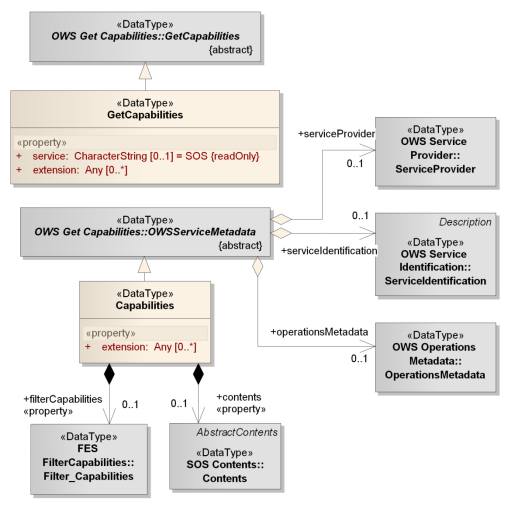
\includegraphics[width=0.7\linewidth]{figs/SOS_2_dataModel_GetCapabilities.PNG}
	\caption{Data model behind the capabilities document of a \ac{sos} \citep{SW:OGC2}}
	\label{fig:Capabilities}
\end{figure}

\subsection{Describe sensor}

\begin{sloppypar}
The \texttt{DescribeSensor} request gives detailed information on a specific sensor. The request is built by taking the \ac{http} address of the \ac{sos} and adding \url{service=SOS\&version=2.0.0\&request=DescribeSensor\&procedure=aprocedure\&proceduredescriptionformat=aformat} where the procedure and procedure description format have to contain values defined in the capabilities document.
\end{sloppypar}

% write about SWE describesensor schema
% http://www.opengis.net/swes/2.0
% http://schemas.opengis.net/swes/2.0/swesContents.xsd

\subsection{Get observation}

Using \texttt{GetObservation} actual measurements can be retrieved. The request is made by taking the \ac{http} address of the \ac{sos} and adding \url{service=SOS\&version=2.0.0\&request=GetObservation}. This returns a response with the default parameters, which can differ from one \ac{sos} to another. To further specify the request, optional paramaters can be added such as: observed property, procedure, feature-of-interest, offering and outputformat. Spatial and temporal filters can be added if these are supported by the service. 

The \texttt{GetObservationByID} request is an extension that let's users retrieve an observation using an identifier that points to a certain observation. 

% write about OM observation schema


\subsection{Get feature of interest}
The \texttt{GetFeatureOfInterest} request allows to retrieve information about the feature of interest of a certain observation. The response can be all features of interest or only ones that are related to a specific observed property, procedure or spatial filter. This request also allows logical operators, for example: \enquote{GetFeatureOfInterest ( observedProperty := temperature AND procedure := thermometerX OR anemometerY )} \citep[p. 40]{SW:OGC2}. The response is a document with `GFI\_features' (\ac{iso} 19109) \citep{GEO:ISO}, which are implemented in the \ac{gml} (\ac{iso} 19136) \citep{GEO:ISO2} by the element gml:AbstractFeature and type gml:AbstractFeatureType \citep[p. 38]{SW:ISO}.

\subsection{Transactional extensions}
It is possible to update the content of a \ac{sos} using transactional request. There are six of these requests that could be implemented: \texttt{InsertCapabilities}, \texttt{InsertObservation}, \texttt{InsertSensor}, \text{DeleteSensor}, \texttt{InsertResultTemplate} and \texttt{InsertResult}. \texttt{InsertCapabilities} allows a request to add data to the capabilities document described in Paragraph \ref{par:capabilities}. The request contains three mandatory parameters and one optional parameter: it is required to have the \texttt{procedureDescriptionFormat}, \texttt{FeatureOfInterestType} and \texttt{ObservationType}. Optionally, \texttt{SupportedEncoding} could be added to the request. An \texttt{InsertCapabilities} should be made in combination with a \texttt{InsertObservation}, \texttt{InsertSensor} or \texttt{InsertResult} request.

A \texttt{InsertResultTemplate} request allows to upload a template for result values. It should contain data about the offering, the observation template, the result structure and result encoding. The actual results can be added later using an \texttt{InsertResult} request. This request is different from the \texttt{InsertObservation} request, as it only inserts the result value of an observation, assuming that the metadata is already present in the \ac{sos}. This is useful when there is limited communication bandwidth and processing power. This request has two mandatory parameters: a pointer to the template and the observation value to be inserted. An \texttt{InsertObservation} request allows observations to be added to a registered sensor system. It also has two mandatory parameters: a pointer to an offering and the observation to be inserted.

Individual sensors can be inserted or deleted using \texttt{InsertSensor} and \texttt{DeleteSensor} requests. For inserting a sensor the following parameters are required: the procedure description format, a procedure description, the observable property, a feature of interest type and an observation type. For deleting a sensor an identifier that points to a specific sensor needs to be passed as a parameter.

\section{Semantic web}

\begin{figure}
	\centering
	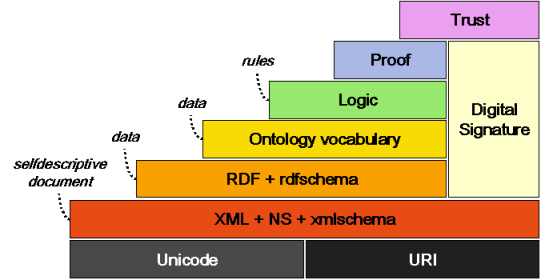
\includegraphics[width=0.7\linewidth]{figs/semanticweb.png}
	\caption{Hierarchy of the semantic web \citep{LD:Koivunen}}
	\label{fig:SemanticWeb}
\end{figure}

\subsection{Resource Description Framework}
For publishing geographic data on the semantic web a conversion of Shapefiles to \ac{rdf} is required. For this the method by \cite{LD:Missier} will be used. First the Shapefile is loaded into a Postgres database with the Postgis extension. After that a Python script retrieves the records from the database. Attributes of the records will be mapped to classes from predefined ontologies. Then the script creates an \ac{rdf} graph and serialises it to a certain \ac{rdf} notation. This is written to a file. The final step is to publish the \ac{rdf} on the web and create a \ac{sparql} endpoint to query the data \citep{LD:Missier}. 

In \ac{rdf} data is stored as so-called `triples'. These triples are structured as: subject, predicate and object \citep{LD:Berners-lee}. The subject and the object are things and the predicate is the relation between these two things. For example, to define a geographic feature such as the municipality of Delft on the semantic web a number of triples can be made. Figure \ref{fig:Triples} shows how Delft can be defined as a municipality with a certain geometry using triples of subject, predicate and object.

\begin{figure}
	\centering
	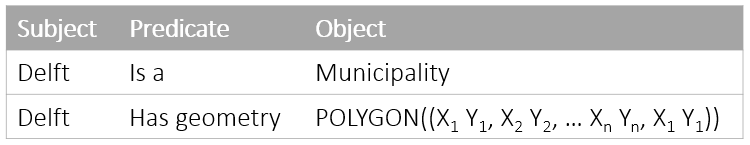
\includegraphics[width=0.7\linewidth]{figs/Triples.png}
	\caption{Triples of object, predicate and subject define Delft as a municipality with a geometry}
	\label{fig:Triples}
\end{figure}

Three types of data can make up these triples \citep{LD:W3C6}. The first type is an \ac{iri}. This is a reference to a resource and can be used for all positions of the triple. A \ac{url} is an example of an \ac{iri}, but \ac{iri}s can also refer to resources without stating a location or how it can be accessed. An \ac{iri} is a generalisation of an \ac{uri}, and also allows non-ASCII characters. In the example of the municipality of Delft, \ac{iri}s can be used to define `Delft' and `Municipality', but also for the predicates `is a' and `has geometry'. The second type of data is a literal. A literal is a value which is not an \ac{iri}, such as strings, numbers or dates. These values can only be used as object in a triple. In the example of Delft, a literal could be used to store the actual geometry of the boundary: POLYGON(( $x_{1},y_{1}$ $x_{2},y_{2}$ ... $x_{n},y_{n}$, $x_{1},y_{1}$ )). A literal value can have a datatype specification \citep{LD:W3C7}. This is added to the literal with the \^{}\^{} symbols, followed by the \ac{iri} of the datatype specification. In Figure \ref{fig:Turtle} the datatype is `geo:wktLiteral'.

Sometimes it is useful to refer to things without assigning them with a global identifier. The third type is the blank node and can be used as an subject or object without using an \ac{iri} or literal \citep{LD:W3C6}.  

\subsection{Notation}
There are a number of different notations for writing down these triples (serialisation), such as \ac{xml} \citep{LD:W3C3}, N3 \citep{LD:W3C5} and Turtle \citep{LD:W3C4}. Turtle will be used in this thesis, because it is commonly used notation which is also relatively easy to read for humans. The DBPedia \ac{iri} is used for the object `Municipality'. The `is a' predicate is represented by a built-in \ac{rdf} predicate which can be written simple as `a'. The second predicate is `hasGeometry' for which the GeoSPARQL \ac{iri} is used. The geometry is a literal in the \ac{wkt} format. Note that the subject is only written once when there are multiple triples with the same subject. Triples that shares the same subject are divided by semicolons. A point marks the end of the last triple with a specific subject.

\begin{figure}
	\centering
	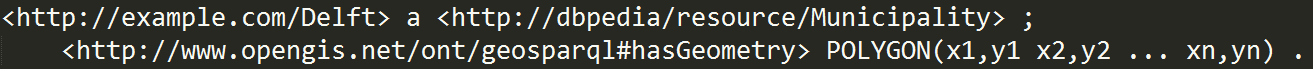
\includegraphics[width=1\linewidth]{figs/Turtle.png}
	\caption{Triples of Figure \ref{fig:Triples} in the Turtle notation}
	\label{fig:Turtle}
\end{figure} 

\subsection{Persistent Uniform Resource Locators}
\acp{url} are an essential part of the web. However, if an \ac{url} changes the existing links towards this \ac{url} are broken. To prevent this \acp{purl} are being used. A \acl{purl} is a \enquote{naming and resolution service for general Internet resources} \citep{LD:PURL}. This allows organisations to change the location of their data without changing the \ac{url} to which can be linked. A \ac{purl} server receives the \ac{url} and redirects the client to the current location of the resource. If the location of the resource 
changes, the server can be informed. It will then redirect clients to the new location (Figure \ref{fig:PURL}).  

\begin{figure}
	\centering
	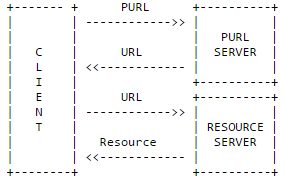
\includegraphics[width=0.6\linewidth]{figs/purl.png}
	\caption{Persistent Uniform Resource Locator (PURL) resolves to the current resource location \citep{LD:PURL}}
	\label{fig:PURL}
\end{figure} 

\section{GeoSPARQL \& stSPARQL}
\label{par:SpatialFilters}
GeoSPARQL \enquote{defines a vocabulary for representing geospatial data in RDF, and it defines an extension to the SPARQL query language for processing geospatial data} \cite[p. xvi]{LD:OGC}. It allows for defining geometric data in \ac{rdf} and performing spatial queries. The \ac{DE9IM} \citep{GIS:9IM} has been implemented to find topological relations between two geometries. GeoSPARQL has been implemented in the `Parliament' \ac{sparql} endpoint \citep{LD:GeoSPARQL}. The Strabon endpoint uses stRDF, which is \enquote{a constraint data model that extends RDF with the ability to represent spatial and temporal data} \cite[p. 425]{SSW:Koubarakis}. The stRDF model can be queried using stSPARQL, which syntax is similar to GeoSPARQL (listing \ref{lst:GeoSPARQL} \& \ref{lst:stSPARQL}). Both extensions of \ac{sparql} use filter expressions to perform spatial operations on \ac{wkt} or \ac{gml} geometries. The definition of geometries and the syntax of the filter expression differ slightly.

\begin{lstlisting}[caption={A GeoSPARQL query to find the names of features that contain a point geometry}, label={lst:GeoSPARQL}]
PREFIX geo: <http://www.opengis.net/ont/geosparql#>
PREFIX geof: <http://www.opengis.net/def/function/geosparql/>
PREFIX foaf: <http://xmlns.com/foaf/0.1/> 

SELECT 
?name
WHERE {
?feature geo:hasGeometry ?geom .
?feature foaf:name ?name.
FILTER (geof:sfContains(?geom,"<http://www.opengis.net/def/crs/EPSG/0/4258> POINT(4.289244 52.027337)"^^geo:wktLiteral))
}
\end{lstlisting}

\begin{lstlisting}[caption={A stSPARQL query to find the names of features that contain a point geometry}, label={lst:stSPARQL}]
PREFIX strdf: <ttp://strdf.di.uoa.gr/ontology#>
PREFIX foaf: <http://xmlns.com/foaf/0.1/> 

SELECT 
?name
WHERE {
?feature strdf:hasGeometry ?geom .
?feature foaf:name ?name.
FILTER (?geom contains "POINT(4.289244 52.027337);<http://www.opengis.net/def/crs/EPSG/0/4258>"^^strdf:WKT)
}
\end{lstlisting}

\section{Ontologies}
When publishing data on the semantic web, ontologies are required to specify what things are and how they relate to other things. The evaluation of observation metadata ontologies by \cite{SW:Hu} is interesting, since it exposes what the relevant aspects are in the process of observation discovery. However, their proposed model focusses mainly on including remote sensing and imagery data in metadata models that were not originally created for this kind of data. The \ac{ssno} is an ontology that clearly describes the process between sensor, stimulus and observation. However, \cite{SSW:Cox4} points out that an important aspect of describing a sensor network is missing in this ontology: the sampling. Also, the om-lite and sam-lite ontologies by \cite{SSW:Cox4} are lightweight ontologies that can be complemented by already existing linked data ontologies. They do not rely on the (heavy) \ac{iso} specifications that date from before the semantic web, unlike the \ac{ssno}. The om-lite and sam-lite ontologies will therefore be used in this thesis. 

 The \ac{sos} has a number of metadata attributes such as the service provider's details (including contact information), its spatial and temporal extent (spatialFiler \& temporalFilter) and the capabilities to query a subset of this extent. It receives data from a sensor which makes observations. An observation can be defined as \enquote{an action whose result is an estimate of the value of some property of the feature-of-interest, obtained using a specified procedure} \citep{SSW:Cox3}.The sensor is placed at a sampling point. The sampling point is part of a sampling feature which intents to resemble the feature-of-interest. In the case of air quality the feature-of-interest is the bubble of air surrounding the sensor, therefore the sampling point equals the feature-of-interest \citep{SDI:INSPIRE2}. The design is that an observation of the sampling feature describes the  feature-of-interest through measuring one of its properties. The measurement procedure is described by a short string of text, input and output parameters and the units of measurement of the ouput. The relation between feature-of-interest and administrative units is added to improve the discovery of sensor data on the semantic web. 

To publish data on the semantic web ontologies are required to specify the different classes and their relations. An ontology for static geographic data has to be connected to an ontology for sensor metadata. From the \ac{uml} diagram in Figure \ref{fig:UML} the classes Observation, Process, ObservedProperty and FeatureOfInterest can be mapped to classes belonging to \ac{owl} for observations \citep{SSW:Cox}. SamplingFeature and Sampling point can be mapped to classes from \ac{owl} for sampling features \citep{SSW:Cox2}. GeoSPARQL can be used for the administrativeUnit class \citep{LD:OGC} and the PROV ontology for the sensor and sensor observation service classes \citep{LD:W3C2}. 

%\begin{figure}
%	\centering
%	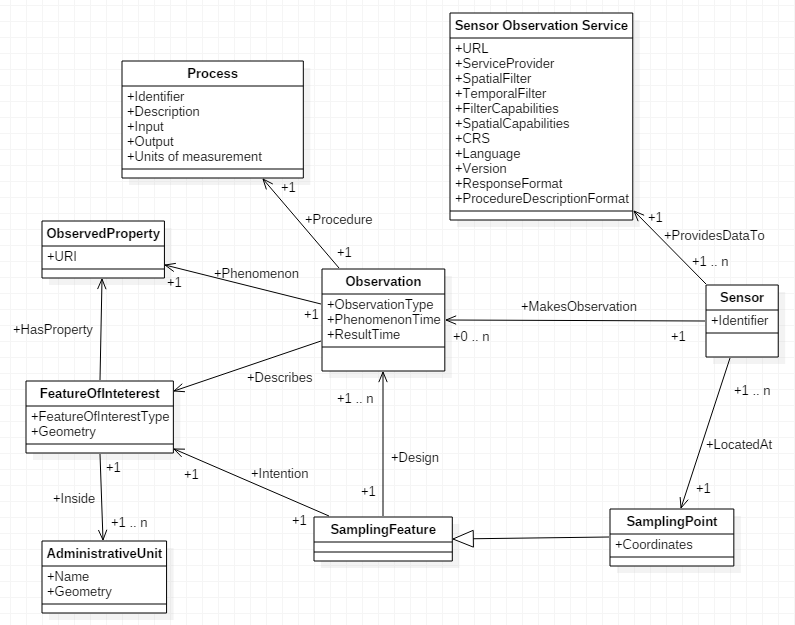
\includegraphics[width=1\linewidth]{UML/UML_Diagram.png}
%	\caption{\ac{uml} diagram of sensor observations service, based on \cite{SSW:Cox3} and \cite{SDI:INSPIRE2}}
%	\label{fig:UML}
%\end{figure}

%\section{Aggregation}
%There are many different ways to aggregate sensor data, for example by taking the minimum value, the maximum value, the average value, the sum, etc. Also, spatial aggregation techniques (based on neighbourhood analysis) can be considered to adjust for spatio-temporal irregularities as mentioned by \cite{SW:Ganesan}. In order to determine which method of aggregation is applicable for a specific kind of sensor data the sensor metadata will contain links to appropriate aggregation methods. However, which methods are appropriate should be based on expert knowledge.

\section{Web Processing Service}
The \ac{ogc} \acl{wps} is a standard interface for making simple or complex computational processing services accessible as web services. Originally, it has been created with spatial processes in mind, but it can also be used to insert non-spatial processing into a web services environment \citep[p. 8]{GEO:OGC}. Via the \ac{wps} jobs can be controlled and monitored, which run certain processes (Figure \ref{fig:WPSmodel}). Similar to \ac{wfs}, \ac{wps} and \ac{sos}, the \ac{wps} has requests for retrieving metadata: \texttt{GetCapabilities} and \texttt{DescribeProcess}. On top of that there are is the \texttt{Execute} request to execute a process, and a number of other requests for various purposes: \texttt{GetStatus}, \texttt{GetResult} and \texttt{Dismiss}. All requests will be briefly described in this paragraph.  

\begin{figure}
	\centering
	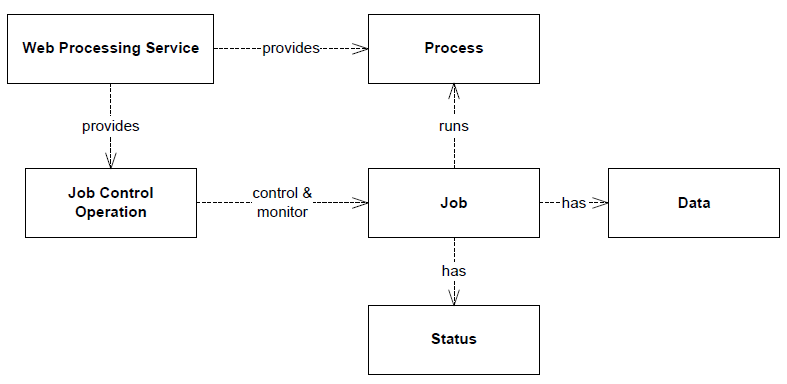
\includegraphics[width=1\linewidth]{UML/WPSmodel.png}
	\caption{Artifacts of the \ac{wps} service model \citep[p. 15]{GEO:OGC}}
	\label{fig:WPSmodel}
\end{figure}

\subsection{Get Capabilities}
All \ac{ogc} web services give an overview of what they have to offer using the so-called \texttt{GetCapabilities} request. The request can be made by taking the \ac{http} address of the \ac{wps} and adding: \url{service=wps&request=getcapabilities}. This returns a document with information about the service metadata, the basic process offerings, and available processes. Figure \label{fig:WPSmodel2} shows the model of this capabilities document. The service identification section of the document gives a description of the service, including the versions that it supports and potential fees or access constraints. The service provider section gives information about the organisation or people who maintain the \ac{wps} and also includes their contact information. The operations metadata lists the different requests that are implemented in this particular \ac{wps} and the \ac{http} addresses to which the GET and POST requests can be send to. The content section of the capabilities document provides an overview of the available process offerings. For every process an identifier, title and description are listed. Optionally an extensions section can be added that describes additional service capabilities. At the end of the document the language section lists the languages that are supported and the default language that is being used. An example of an capabilities document can be found in Appendix \ref{app:wpsCapabilities}  

\begin{figure}
	\centering
	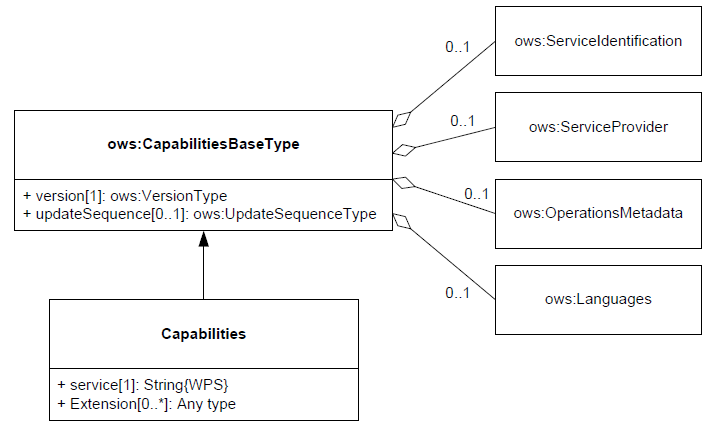
\includegraphics[width=1\linewidth]{UML/WPSmodel2.png}
	\caption{\ac{uml} model of WPS capabilities document \citep[p. 70]{GEO:OGC}}
	\label{fig:WPSmodel2}
\end{figure}

\subsection{Describe Process}
A more detailed description of a process listed in the capabilities document of the \ac{wps} can be retrieved using the \texttt{DescribeProcess} request. This request requires the identifier of the process to be passed as a parameter. Optionally, a specific language can be requested for the response document (from the list of available languages in the capabilities document). The process description includes information about input parameters and output data, such as their identifiers, data type, mime types or default values. A describe sensor request can be made by putting the base address of the \ac{wps} and adding: \url{service=wps&version=1.0.0&request=describeprocess&identifier=an_identifier} where the version parameter should be in accordance with the supported version(s) from the capabilities document and the identifier should be taken from the process offerings section of the capabilities document. An example of an describe sensor response document can be found in Appendix \ref{app:wpsDescribe}  


\subsection{Execute}
A \ac{wps} process can be started using the \texttt{Execute} request. To make this request the \ac{http} address of the \ac{wps} is extended with: \url{service=wps&version=1.0.0&request=execute&identifier=GetSensors} where the version parameter should be in accordance with the supported version(s) from the capabilities document and the identifier should be taken from the process offerings section of the capabilities document. 

Depending on the individual requirements of the process input parameters can be added using \url{&DataInputs=[parameterName1=value1;parameterName2=value2]}. The parameter names are defined in the describe process response document, as well as the allowed values for each parameter. There are two kinds of input parameters that can be put in a \texttt{Execute} request: literal and complex data inputs. Literal data inputs can be a string of characters in consisting of different data types (e.g. Double, Integer, String), a given value range, and associated units (e.g. meters, degrees Celsius) \citep[p. 36]{GEO:OGC}. 

Complex data inputs are made for inputting complex vector-, raster- or other kind of data.  

If the process finishes successfully an execute response document is retrieved. This document contains

An example of an execute response document can be found in Appendix \ref{app:wpsExecute}

\subsection{Other requests}
\texttt{Get Status}

\texttt{Get Result}

\texttt{Dismiss}
